\documentclass[border=3pt,tikz]{standalone}
\usepackage{amsmath}
\usetikzlibrary {arrows.meta}
\begin{document}
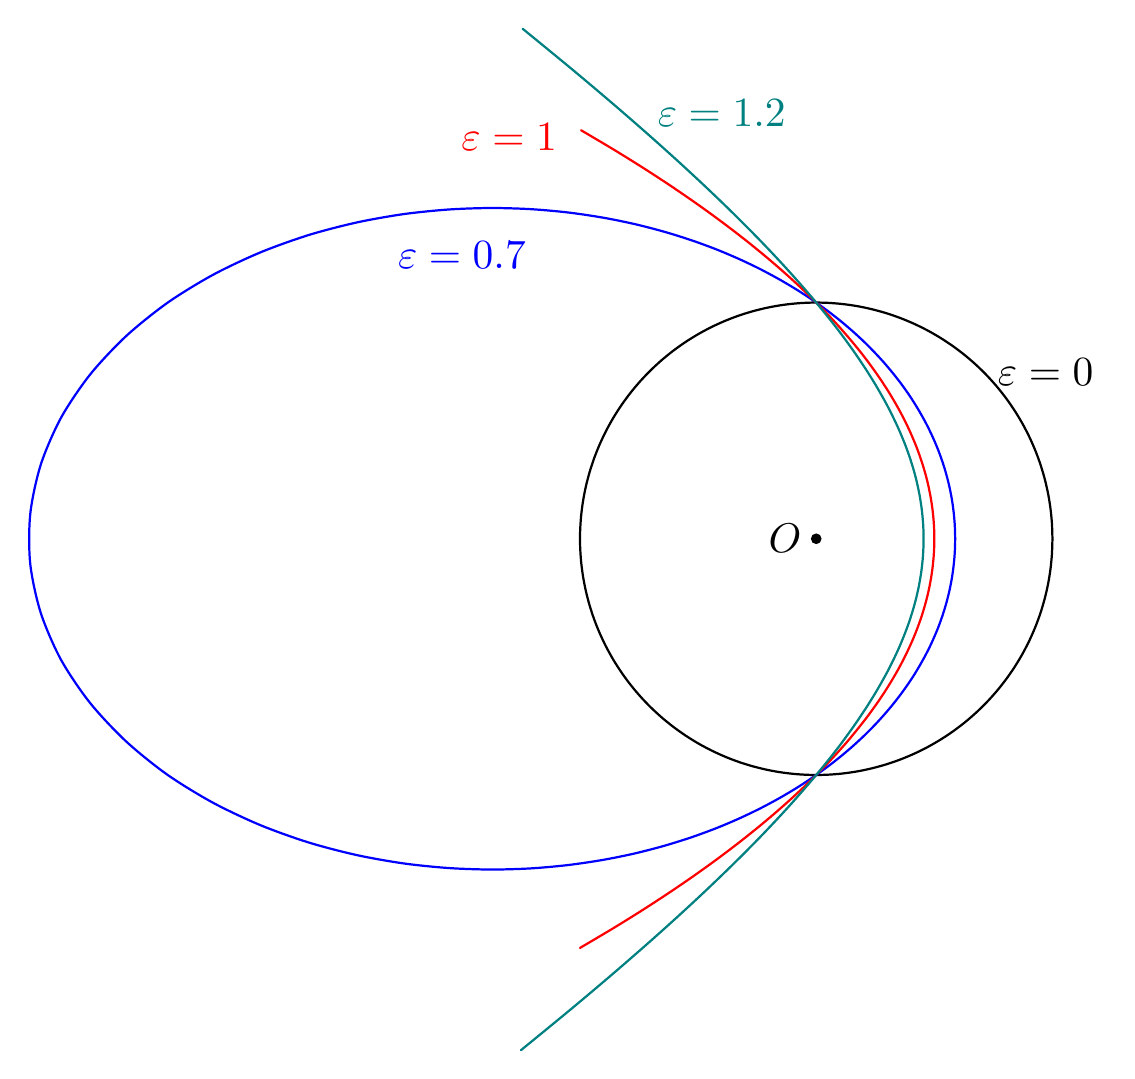
\begin{tikzpicture}[line cap=round, scale=3]

    \filldraw[](0,0) circle (0.02);
    \node[left, scale = 1.5] at (0, 0) {$O$};
    
    \draw[black, thick] plot[variable=\t,domain=0:2*pi, samples=100, smooth,thick] ({cos(\t r)},{sin(\t r)});
    \node[right, scale=1.5] at (0.707, 0.707) {$\varepsilon =0$};
    
    \draw[blue, thick] plot[variable=\t,domain=0:2*pi, samples=100, smooth,thick] ({cos(\t r)/(1+0.7 * cos(\t r))},{sin(\t r)/(1+0.7 * cos(\t r))});
    \node[blue, scale = 1.5] at (-1.5, 1.2) {$\varepsilon = 0.7$};
    
    \draw[red, thick] plot[variable=\t,domain=-2*pi/3:2*pi/3, samples=100, smooth,thick] ({cos(\t r)/(1+  cos(\t r))},{sin(\t r)/(1 +  cos(\t r))});
    \node[red, scale = 1.5] at (-1.3, 1.7) {$\varepsilon = 1$};
    
    \draw[teal, thick] plot[variable=\t,domain=-2*pi/3:2*pi/3, samples=100, smooth,thick] ({cos(\t r)/(1.0+ 1.2* cos(\t r))},{sin(\t r)/(1.0 + 1.2* cos(\t r))});
    \node[teal, scale = 1.5] at (-0.4, 1.8) {$\varepsilon = 1.2$};
    \end{tikzpicture}
\end{document}